\chapter{Problem description}\label{chap:Problem description}
%第一段：summary of the problem + 优先描述multi-deep layout的布局constraint，因为这个约束在初始化和后续调度过程都起到了重要作用。 本problem description后续关注的重点将是解释：1.dynamic 2. retrieval and relocation scheduling problem。
This work investigates a dynamic retrieval and relocation scheduling problem in a shuttle-based variant of multi-deep AVS/RSs, namely multi-deep Shuttle-Based Storage and Retrieval Systems (SBS/RSs). Specifically, this work focuses on the scheduling problem within a fixed tier served by a single shuttle in a tier-captive multi-deep SBS/RS, considering dynamic order-driven target item activation, with the objective of minimizing total tardiness. 

% 第1.5段，然后我补充了practial这部分，因为这个是有现实要求和意义的。你之前就抛一个名词太单薄了。（而且这个名词compact storage lane configuration是专有名词吗？）
To reflect the compact storage lane configuration constraint with practical multi-deep warehouse operations, items in each storage lane are stored contiguously from the deep end, without empty locations between stored items. Accordingly, in any partially occupied storage lane, all occupied storage locations must be located deeper than all empty storage locations. 


%第二段：介绍初始仓库布局，并具体解释了第一段介绍的约束是如何影响初始布局的。从仓库布局角度解释了为何本任务是retrieval and relocation而非单纯的retrieval。同时将初始target item描述为被已知订单激活，也完善后续的动态订单激活逻辑。后续反正都要说激活，你这里先说了就显得很重复。

In the initial state, the warehouse is not fully occupied. The initial items are distributed randomly across storage locations subject to the above compact storage lane configuration constraint. A subset of the initial items is activated by initially known orders as target items with individual due dates, while the remaining initial items are non-target items. 



%第三段：简单（不涉及DRL AGENT，只介绍操作本身）介绍retrieval and relocation operation，并具体解释了第一段介绍的约束是如何影响的relocation调度过程。这部分的内容有点太反复说了，比如这个unload it就出现了两次。然后still compact lane这个没必要在这说，这里就说可行的empty location就行了，具体啥是可行，可以留到DRL部分介绍action space 的地方再说。

This random initial configuration may place target items at different storage depths, with some targets located behind one or more non-target items. Before such a target can be retrieved, the blocking non-target items must first be relocated. At each decision point, the shuttle either retrieves an accessible target item by transporting it to the I/O point or relocates an accessible blocking non-target item to a feasible empty location in another storage lane.

%第四段：介绍何为dynamic：stochastic order arrival驱动的target item activation。继而引出本文的dynamic order-driven target item activation机制的建模方法：global Poisson arrival process。最后给出整个调度任务的结束条件。这里order和item的关系没有明确说明。容易产生混乱
During the scheduling process, orders may arrive at any discrete time step, and each order may contain multiple item requests. Each item request converts one currently non-target item into a new target item and assigns it an individual due date. To model the stochastic arrival of such item requests, this work adopts a global Poisson arrival process, which is used to describe the number of random arrival events occurring independently in non-overlapping time intervals. 

Fig. \ref{fig:flowchart of item activation} illustrates the general logic of this dynamic order-driven target item activation. Specifically, let $X_t$ denote the number of non-target items requested to be activated by orders arriving at discrete time step $t$. Then, $X_t$ follows a Poisson distribution, and its probability mass function (PMF) is given by:
\begin{equation}
\Pr(X_t=k)=\frac{e^{-\lambda}\lambda^k}{k!}, \quad k \in \mathbb{N}_{0}
\end{equation}
where the non-negative integer $k$ denotes one possible value of the number of items requested to be activated in this time step, and the parameter $\lambda$ denotes the expected number of activations per time step. Let $\mathcal{N}_t$ denote the set of all non-target items in the warehouse at discrete time step $t$. Then, the actual number of activated items $A_t$ is given by:
\begin{equation}
A_t=\min\{X_t,|\mathcal{N}_t|\}.
\end{equation}
After $A_t$ is determined, the system uniformly samples $A_t$ non-target items from the set $\mathcal{N}_t$ without replacement, activates them as new target items, and randomly assigns individual due dates to them.  

% 这里需要增加说明，为什么需要pre define的activate window和number，就在assumption里写一句不够。而且这算是机制，和其他的assumption也不一样。
To ensure a finite dynamic activation horizon and comparable scheduling episodes across problem instances, a maximum activation time window and a threshold for the number of remaining non-target items are predefined. The target item activation process terminates when either the activation time window expires or the number of remaining non-target items falls below the predefined threshold. Once either condition is met, no further target items are activated.


\begin{figure}[!htbp]
\centering
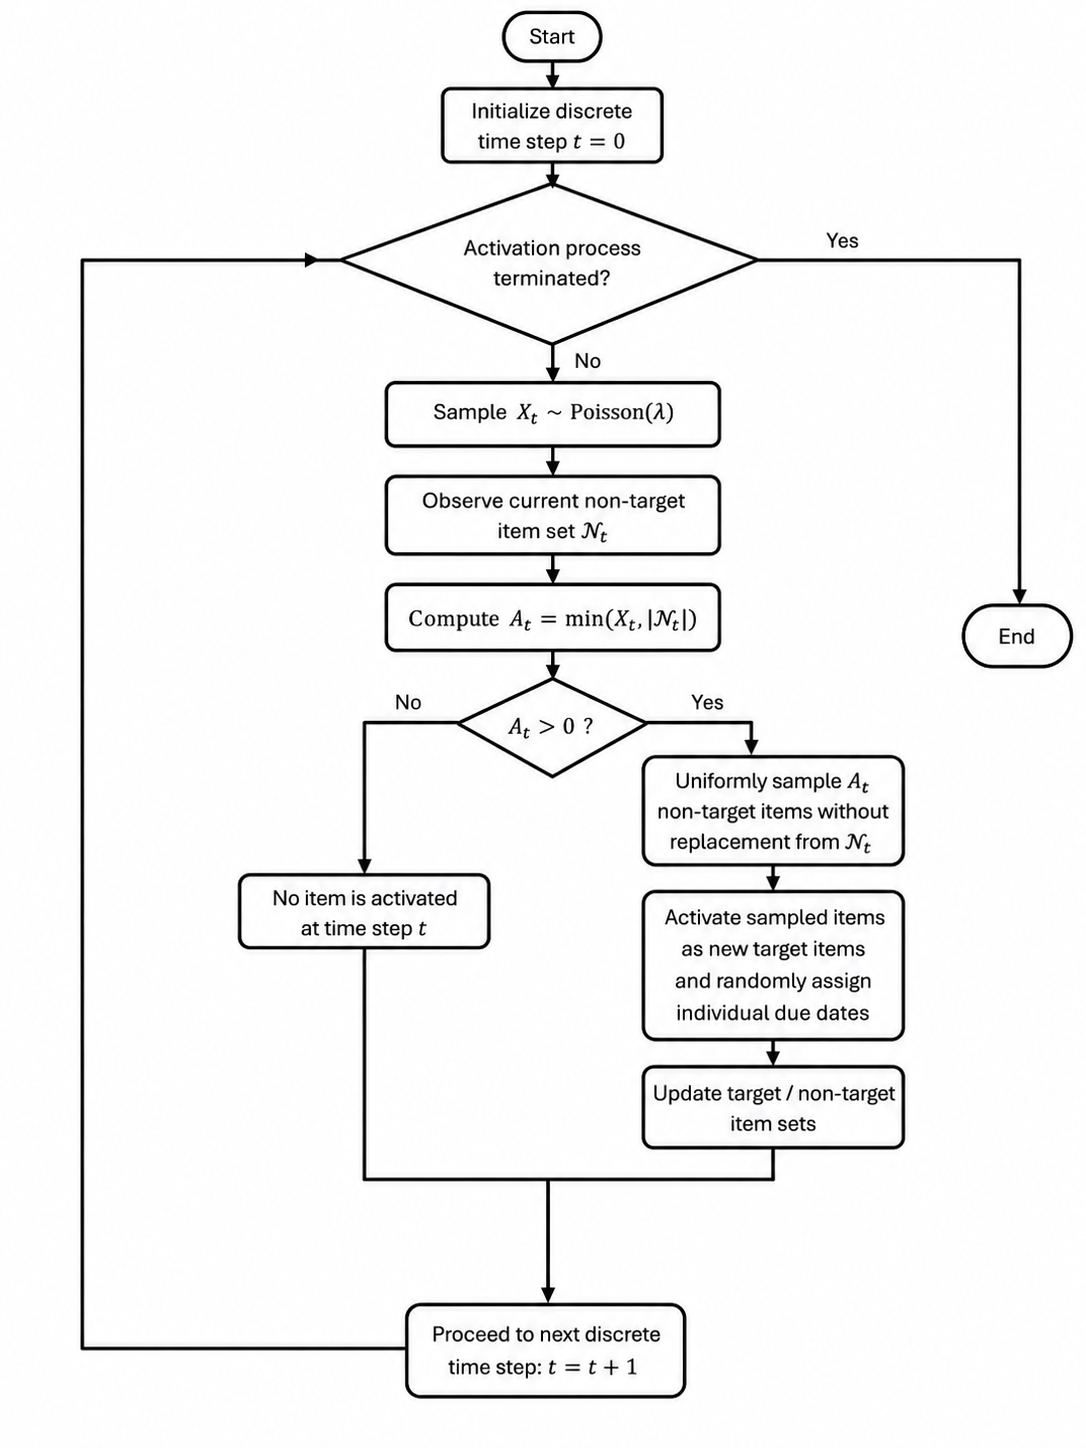
\includegraphics[width=.7\linewidth]{graphics/fig3.png}
\caption{Flowchart of dynamic order-driven target item activation}
\label{fig:flowchart of item activation}
\end{figure}
%第五段：介绍整个调度任务的优化目标及其对应的数学表达式
The optimization objective of this work is to minimize the total tardiness of all activated target items. Let $\mathcal{T}$ denote the set of all activated target items during the entire scheduling process. For any target item $i\in\mathcal{T}$, let $D_i$ denote its due date and let $C_i$ denote the discrete time step at which it completes unloading at an I/O point. Then, the tardiness of this target item is defined as:
\begin{equation}
T_i=\max\{0,C_i-D_i\}.
\end{equation}
Therefore, the mathematical expression for minimizing total tardiness is given by:
\begin{equation}
\min\sum_{i\in\mathcal{T}}T_i
=
\min\sum_{i\in \mathcal{T}}\max\{0,C_i-D_i\}.
\end{equation}
%第六段：介绍本文的简化假设
To clearly focus on the objective of this work, we have introduced the following assumptions:
\begin{enumerate}
    \item This work adopts a discrete-time model. Each one-step movement of the shuttle between two adjacent locations, each loading operation, and each unloading operation consumes one time step.
    
    \item This work considers only the scheduling problem within a fixed tier. Lifts, conveyors, and other auxiliary resources are assumed to be sufficiently configured. Therefore, cross-tier transportation, waiting for auxiliary resources are not considered.
    
    \item All items have the same size, each storage location can store at most one item, and the shuttle can transport at most one item at each retrieval or relocation operation. After a target item is unloaded at an I/O point, it will be immediately removed from the system and regarded as retrieved.
    
    \item The dynamic target item activation process terminates when either of the following conditions is triggered: the current time step exceeds the predefined activation time window, or the number of remaining non-target items in the warehouse falls below a predefined threshold.
\end{enumerate}

